\section{Math 202a - HW5 - Dan Davison - \texttt{ddavison@berkeley.edu}}

% 5. You have the right idea here. Since a Cantor set contains no interval, it is not too hard to always put the new Cantor set inside the intervals missed by the older Cantor sets, so their intersection is trivial. This can then be used rather cleverly to prevent their union from containing an interval. (-6)
% Aidan Backus, Oct 14 at 8:20am
% 2. Your argument almost works but runs into the subtlety that \infty is not < \infty, in case that \mu(E) = \infty (in which case, if G is connected, it will follow that \mu(I_i) = \infty). This can be easily fixed by exploiting \sigma-finiteness. (-2)
% Aidan Backus, Oct 15 at 12:20pm
% 1. 10 2. 8 5. 5 6. 10
% Ian Francis, Oct 16 at 11:41am


\begin{mdframed}
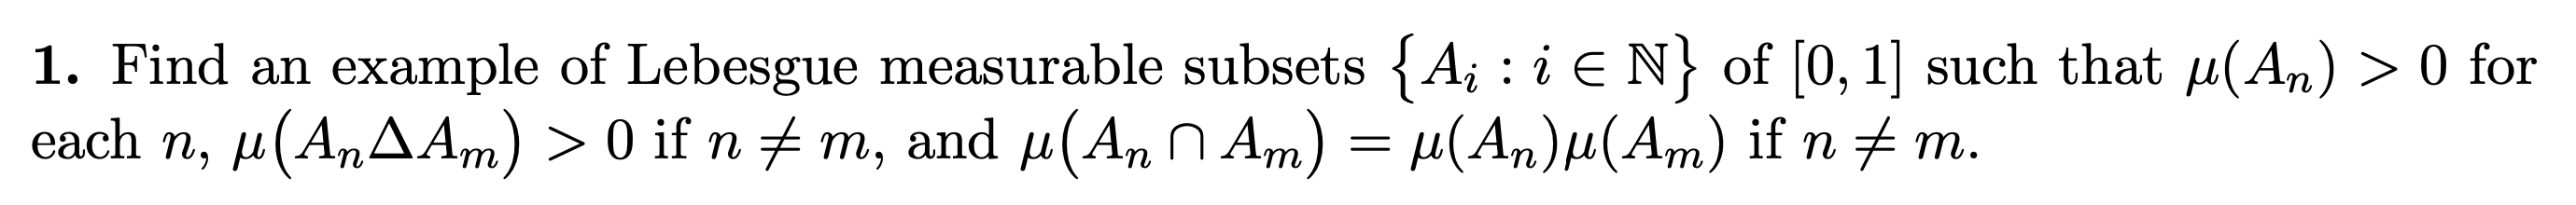
\includegraphics[width=400pt]{img/analysis--berkeley-202a-hw05-781b.png}
\end{mdframed}


\begin{definition*}
  Let $d_n(\om)$ be the $n$-th digit in the binary expansion of $\om$. If $\om$ has two equivalent binary
  expansions, we use the non-terminating one. Define
  \begin{align*}
    A_n := \{\om ~:~ d_n(\om) = 0, ~ \om \in [0, 1]\}.
  \end{align*}
  Thus, for example, $A_1 = (0, 1/2]$ and $A_2 = (0, 1/4] \cup (1/2, 3/4]$.
\end{definition*}

\begin{claim*}
  $A_n$ is Lebesgue measurable for all $n \in \N$.
\end{claim*}

\begin{proof}~\\~\\
  Since $A_n$ is a finite union of intervals of the form $(a, b]$, and since
  \begin{align*}
    (a, b] = \bigcap_{n=1}^\infty (a, b + n^{-1}),
  \end{align*}
  we see that $A_n$ is a finite union of open intervals in $[0, 1]$, hence in the Borel $\sigma$-algebra
  on $[0, 1]$, and hence in the Lebesgue $\sigma$-algebra on $[0, 1]$.
\end{proof}

\begin{claim*}
  $\mu(A_n) > 0$ for all $n$.
\end{claim*}

\begin{proof}~\\~\\
  Note that $(0, 2^{-n}] \subseteq A_n$, therefore by monotonicity of measure
  \begin{align*}
    \mu(A_n) \geq \mu((0, 2^{-n}]) = 2^{-n} > 0.
  \end{align*}
\end{proof}

\begin{claim*}
  $\mu(A_n \Delta A_m) > 0$ if $n \neq m$.
\end{claim*}

\begin{proof}~\\~\\
  Let $m \neq n$ and suppose without loss of generality that $m < n$.

  Then $(0, 2^{-m}] \subseteq A_m$ and also $(2^{-n}, 2^{-(n+1)}] \subset A_m$.
  But $(2^{-n}, 2^{-(n+1)}] \subset A_n^c$ and has non-zero measure, therefore $\mu(A_n \Delta A_m) > 0$.
\end{proof}

\begin{claim*}
  $\mu(A_n \cap A_m) = \mu(A_n)\mu(A_m)$ if $n \neq m$.
\end{claim*}

\begin{proof}~\\~\\
  Let $m \neq n$ and suppose without loss of generality that $m < n$.

  Recall that half of the rank-$i$ dyadic intervals are contained within $A_i$ (those corresponding to
  the $i$-th digit being zero). Therefore $A_i$ is the union of $2^{i-1}$ intervals each of length $2^{-i}$,
  and we have for all $i$
  \begin{align*}
     \mu(A_i) = 2^{i-1}2^{-i} =\frac{1}{2},
  \end{align*}
  therefore $\mu(A_n)\mu(A_m) = \frac{1}{4}$.

  So we need to show that $\mu(A_n \cap A_m) = \frac{1}{4}$.

  Recall that $A_m$ is the union of $2^{m-1}$ dyadic intervals. Let $I$ be one of these intervals. Recall
  that $I$ is partitioned exactly by $2^{n-m}$ rank-$n$ dyadic intervals, each of length $2^{-n}$, and that one
  half of these consist entirely of real numbers with $m$-th digit zero, while the other half have $m$-th digit
  one. Therefore,
  \begin{align*}
    \mu(A_n \cap A_m) = 2^{m-1}2^{n-m}2^{-n}2^{-1} = \frac{1}{4}.
  \end{align*}
\end{proof}
\newpage
\begin{mdframed}
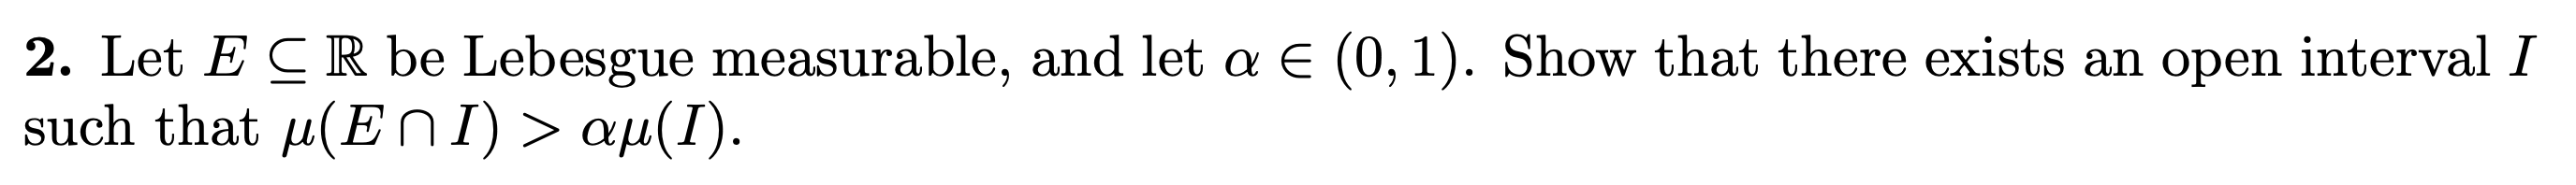
\includegraphics[width=400pt]{img/analysis--berkeley-202a-hw05-2e34.png}\\
It is specified also that $\mu(E) > 0$.
\end{mdframed}

\begin{quote}
  Your argument almost works but runs into the subtlety that $\infty$ is not $< \infty$, in case
  that $\mu(E) = \infty$ (in which case, if $G$ is connected, it will follow that $\mu(I_i) = \infty$). This
  can be easily fixed by exploiting $\sigma$-finiteness. (-2)
\end{quote}

\begin{proof}~\\~\\
  Let $E \subseteq \R$ be Lebesgue measurable and fix $\alpha \in (0, 1)$.

  Set $\eps = \mu(E)\frac{1 - \alpha}{\alpha}$. Since $E$ is Lebesgue measurable there exists an open set $O$
  such that $E \subseteq O$ and $\mu(O \setminus E) < \eps$. Therefore
  \begin{align*}
    \mu(O)
    &= \mu(O \cap E) + \mu(O \setminus E) \\
    &= \mu(E) + \mu(O \setminus E) \\
    &< \mu(E) + \mu(E)\frac{1 - \alpha}{\alpha} \\
    &= \mu(E)/\alpha,
  \end{align*}
  that is,
  \begin{align*}
    \mu(E) = \mu(E \cap O) > \alpha\mu(O).
  \end{align*}
  Now, write $O$ as a countable union of disjoint open intervals $O = \bigcup_{i=1}^\infty I_i$. Note that
    \begin{align*}
    \mu(E)
    &= \mu\Big(E \cap \big(\bigcup_{i=1}^\infty I_i\big)\Big) \\
    &= \mu\Big(\bigcup_{i=1}^\infty E \cap I_i\Big) \\
    &= \sum_{i=1}^\infty \mu(E \cap I_i).
  \end{align*}
  Also $\mu(O) = \sum_{i=1}^\infty \mu(I_i)$. Therefore we have
  \begin{align*}
    \mu(E) = \sum_{i=1}^\infty \mu(E \cap I_i) > \alpha \sum_{i=1}^\infty \mu(I_i).
  \end{align*}
  To see that this implies the desired result, suppose for a contradiction
  that $\mu(E \cap I_i) \leq \alpha \mu(I_i)$ for all $i$. Then we have
  \begin{align*}
    \sum_{i=1}^\infty \mu(E \cap I_i) \leq \alpha \sum_{i=1}^\infty \mu(I_i),
  \end{align*}
  a contradiction.

  Therefore there exists an open interval $I_i$ such that $\mu(E \cap I_i) > \alpha \mu(I_i)$.
\end{proof}


\newpage
\begin{mdframed}
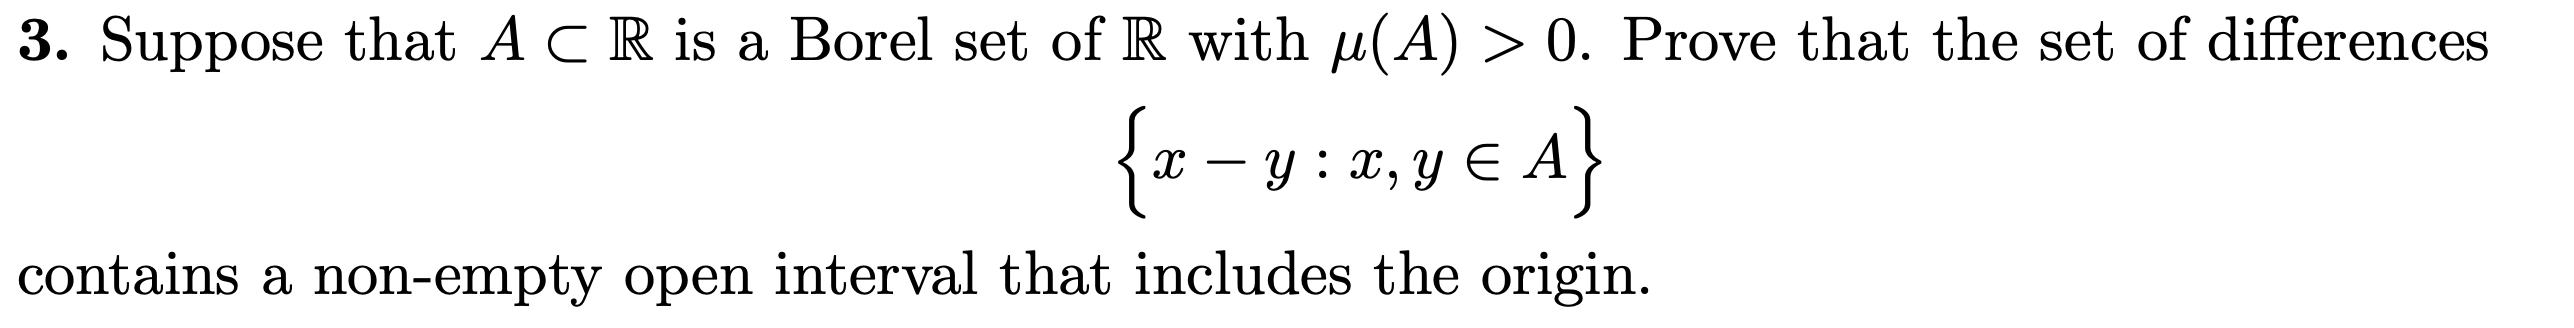
\includegraphics[width=400pt]{img/analysis--berkeley-202a-hw05-ad8b.png}
\end{mdframed}

\url{https://www.wikiwand.com/en/Steinhaus_theorem}

\begin{remark*}
  If $A$ includes an open interval $(a, b)$ then the result easily follows on considering the
  map $z:(a, b)^2\to [a-b, b-a]$. But $A$ may not include any interval and still have positive measure: the
  generalized Cantor sets provide examples.
\end{remark*}

\begin{remark*}
  I tried for a few hours to answer this without hints but in the end followed the sequence of hints provided
  at \url{https://math.stackexchange.com/a/1079520/397805}.
\end{remark*}


\begin{intuition*}
  The crux of this proof is that we translate the statement about the set of differences into a statement about
  what happens when we form the union of the ``inner​'' set $F$ with a version of itself shifted by a small
  amount. The hypothesis that the set of distances includes no interval around the origin corresponds to a
  requirement that this union is of two disjoint sets and therefore that the measure of the union is twice the
  measure of the original. But this reveals a contradiction since the union is itself a subset of the ``outer​''
  set $G$.
\end{intuition*}

\begin{proof}~\\~\\
  Let $A \subset \R$ be a Borel set of $\R$ with $\mu(A) > 0$.

  Let $\eps > 0$.

  Let $F \subseteq A$ be a closed set such that $\mu(A \setminus F) < \epsilon/2$, and let $G \supseteq A$ be
  an open set such that $\mu(G \setminus A) < \epsilon/2$. Thus we have $F \subseteq A \subseteq G$
  and $\mu(G) - \mu(F) < \eps$.

  Let $d = \inf \{ x - x' ~:~ x \in F, x' \in G^c\}$.

  Fix $\delta \in (0, d)$.

  Suppose for a contradiction that there exists $r$ such that $|r| < \delta$ and $F \cap (F + r) = \emptyset$.

  Then $\mu(F \cap (F + r)) = \mu(F) + \mu(F + r) = 2\mu(F)$ by finite additivity and translation invariance of
  measure. Also note that $F \cup (F + r) \subseteq G$, hence $\mu(F \cap (F + r)) \leq \mu(G)$.

  Therefore $\mu(F) \leq \frac{1}{2}\mu(G)$.

  But recall that we have $\mu(G) - \mu(F) < \eps$, therefore $\mu(G) < \eps + \frac{1}{2}\mu(G)$ or
  equivalently $\mu(G) < 2\eps$.

  Since $A \subseteq G$ we then have $\mu(A) < 2\eps$. But $\mu(A)$ is fixed whereas $\eps$ can be chosen
  arbitrarily small, so this is a contradiction.

  Therefore, no such $r$ exists. This means that for all $r$ with $|r| < \delta$, there exist $x, x' \in F$
  such that $x - x' = r$. And since $F \subseteq A$, we have proven the desired result.
\end{proof}


\newpage
\begin{mdframed}
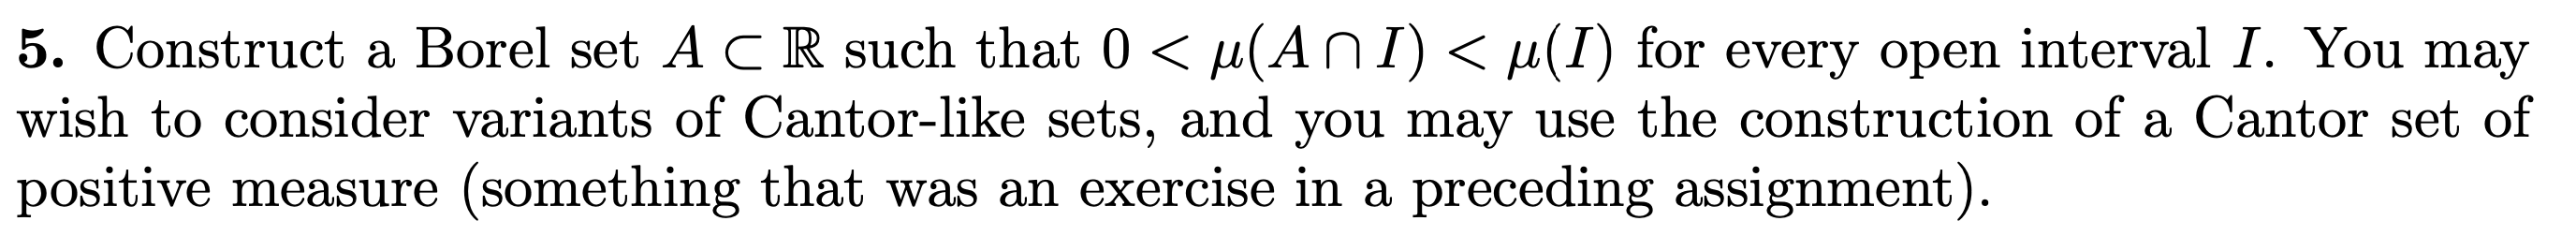
\includegraphics[width=400pt]{img/analysis--berkeley-202a-hw05-40cd.png}
\end{mdframed}

\begin{proof}~\\~\\
  (INCOMPLETE)

  Note that every open interval $I \subseteq \R$ contains a rational number.

  We will construct a set $A$ with positive measure using Cantor-like sets with the following properties:
  \begin{enumerate}
  \item $\Q \subset A$
  \item No interval is a subset of $A$
  \end{enumerate}
  Clearly, (1) has the consequence that $A \cap I \neq \emptyset$ for every open interval $I$. We will show
  that moreover $A$ has the required property: $0 < \mu(A \cap I) < \mu(I)$ for every open interval $I$.

  Let $q_1, q_2, \ldots$ be an enumeration of all distinct rational numbers.

  Fix the total measure $a \in (0, 1)$. For every $i \in \N$ we will construct a Cantor-like set $A_i$ which
  has measure $a/2^i$, contains $q_i$, and is disjoint from $A_j$ for all $j \in \N$ where $i \neq j$.

  Then we define $A := \bigcup_{i=1}^\infty A_i$.

  That's my hope anyway. We now need to specify a construction of these Cantor sets and prove that, when we
  form their union, we do not create any intervals. That's slightly reminiscent of question 3, where the proof
  involves showing that we {\it do} create an interval when we form the union of a certain set with a translated
  version of itself. However, I haven't managed to complete this proof.
\end{proof}


\newpage
\begin{mdframed}
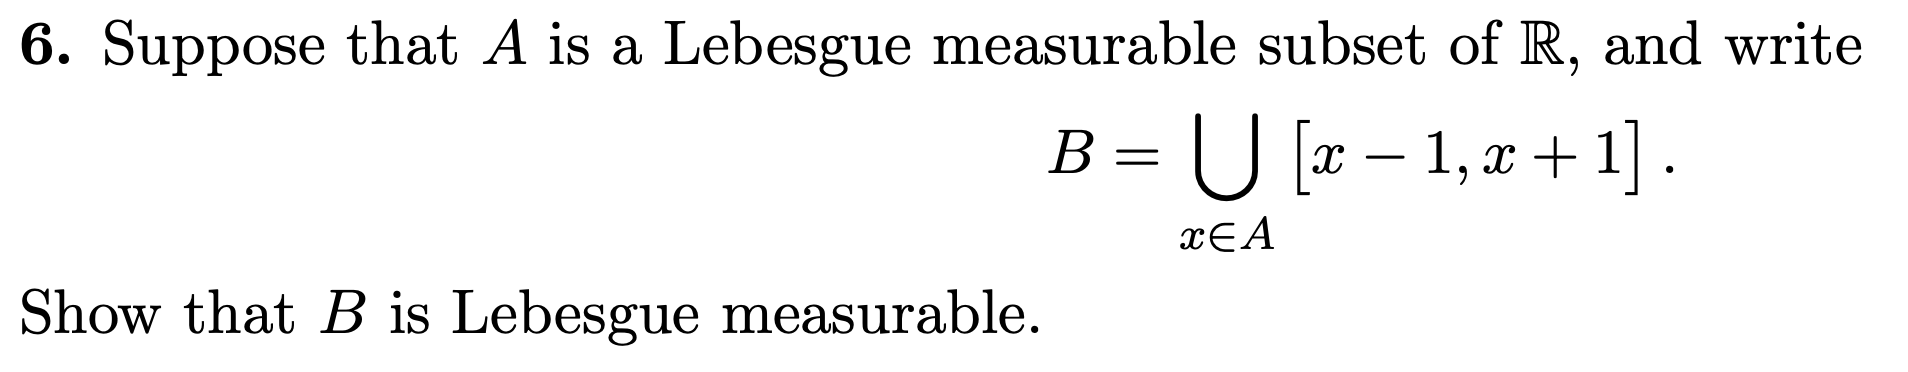
\includegraphics[width=400pt]{img/analysis--berkeley-202a-hw05-3d2c.png}
\end{mdframed}

\begin{proof}
  Let $\mc I := \big\{[x-1, x+1] ~:~ {x \in A} \big\}$, so that $\mc B = \bigcup_{I \in \mc I} I$, and define
  \begin{align*}
    I_x := \bigcup_{I \in \mc I, x \in I} I.
  \end{align*}
  Note that $I_x$ is a union of intervals all of which contain the point $x$ and hence is also an interval.

  Let $q_1, q_2, \ldots \in \Q$ be an enumeration of the rationals.

  Since every $I \in \mc I$ contains a rational (in fact, it contains a countable infinity of rationals), we
  have that for all $I \in \mc I$ there exists $q$ such that $I \subseteq I_q$. Therefore
  \begin{align*}
    \bigcup_{i} I_{q_i} = \bigcup_{I \in \mc I} I = \mc B.
  \end{align*}
  Thus we have written $\mc B$ as a countable union of intervals. These intervals may be open, closed or
  half-open. Recall (Bass proposition 2.8) that the Borel $\sigma$-algebra may be generated by a countable
  collection of open intervals, or of closed intervals, or of half open intervals. Therefore $\mc B$ is in the
  Borel $\sigma$-algebra, therefore $\mc B$ is Lebesgue-measurable.
\end{proof}
